\section{検証結果}
V字モデルに従って、実装部分に関するテストを行った。次に、それぞれに対してテストを行うことで、要件を満たしているかどうかを確認した。以下にそれぞれのテストの項目結果を表で示す。

\subsection{単体テスト}
3章では、単体テスト項目を作成して、詳細設計を満たしているかどうかを確認した。3章のテスト項目に対して、確認結果と、確認日というカラムを加えた。テスト項目に対して検証が成功すれば〇を付ける。検証が失敗した場合は×を付ける。確認日は、テスト項目を検証した日時を記入した。

\subsection*{サーバ通信}
サーバ通信の検証で行った単体テスト項目の検証結果を以下の表\ref{server_test_result}に示す。%始めに、RaspberryPiとサーバの通信にかかわる項目をテストした。

\begin{table}[htbp]
\centering
\caption{サーバ通信単体テストの項目}
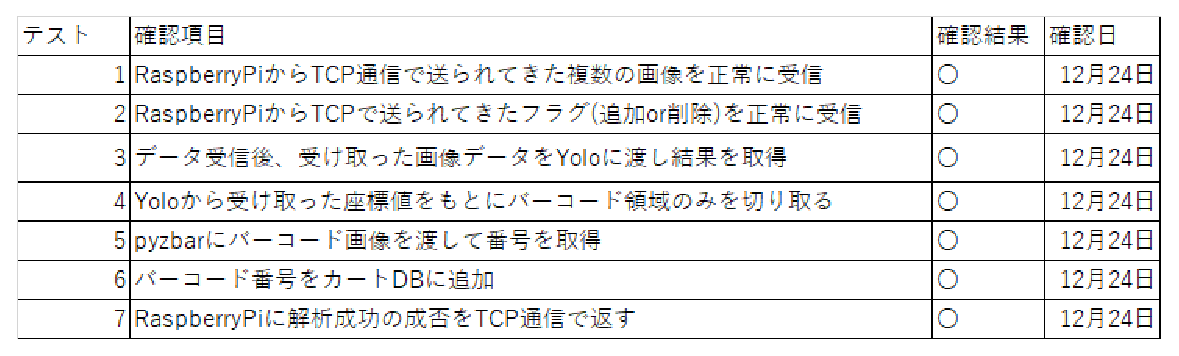
\includegraphics[width=14cm]{./pic/result/server_test_result.eps}
\label{server_test_result}
\end{table}


\subsection*{Yoloによるバーコード領域検知}
Yoloにおけるバーコード領域検知の検証で行った、単体テスト項目の検証結果を以下の表\ref{yolo_test_result}に示す。%Yoloを使用して、画像からバーコード画像のみを切り取ることができるか、テストを行った。まずは、Windows10でGPUオプションのYoloを動作させる必要があったためコンパイルを行った。次に、バーコード画像を識別するような学習済みデータは公開されていなかったため、サンプル画像を集めて学習を行った。そして、本研究では主にPythonを使用してシステムを開発していたので、YoloをPython経由で実行できるようにした。

\begin{table}[htbp]
\centering
\caption{Yoloによるバーコード領域検知単体テストの項目}
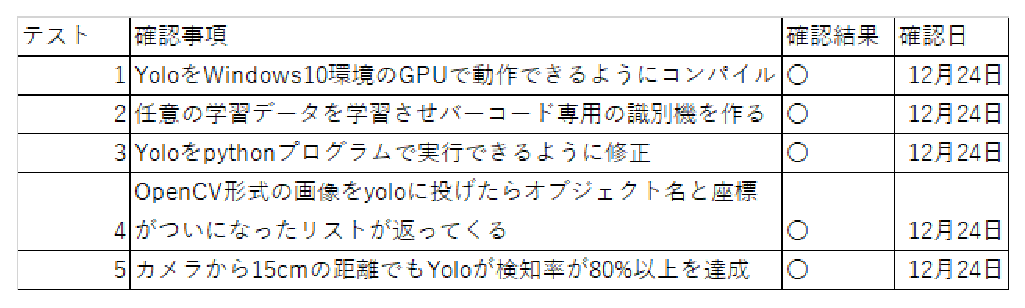
\includegraphics[width=14cm]{./pic/result/yolo_test_result.eps}
\label{yolo_test_result}
\end{table}

\newpage

\subsection*{DBを使用した商品情報の管理}
DBを使用した、商品情報の管理の単体テスト項目の検証結果を以下の表\ref{table_test_result}に示す。

\begin{table}[htbp]
\centering
\caption{DBテーブル単体テストの項目}
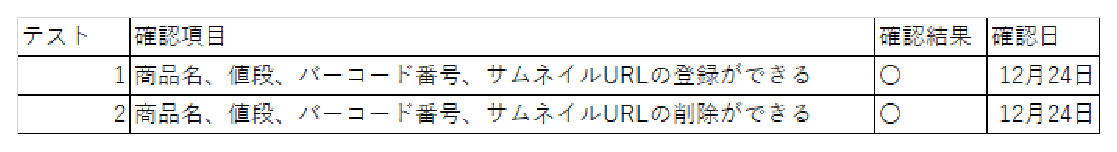
\includegraphics[width=15cm]{./pic/result/table_test_result.eps}
\label{table_test_result}
\end{table}

\subsection*{決済システム}
決済システムにおける単体テスト項目の検証結果を、以下の表\ref{db_test_result}に示す。
%決済システムは、ユーザが決済を行うときに動作する。ユーザが商品を出し入れする時点で、購入予定商品の情報がカゴDBに格納されているため、決済時にカゴの中にある商品を1つずつスキャンする必要はない。

\begin{table}[htbp]
\centering
\caption{決済システム単体テストの項目}
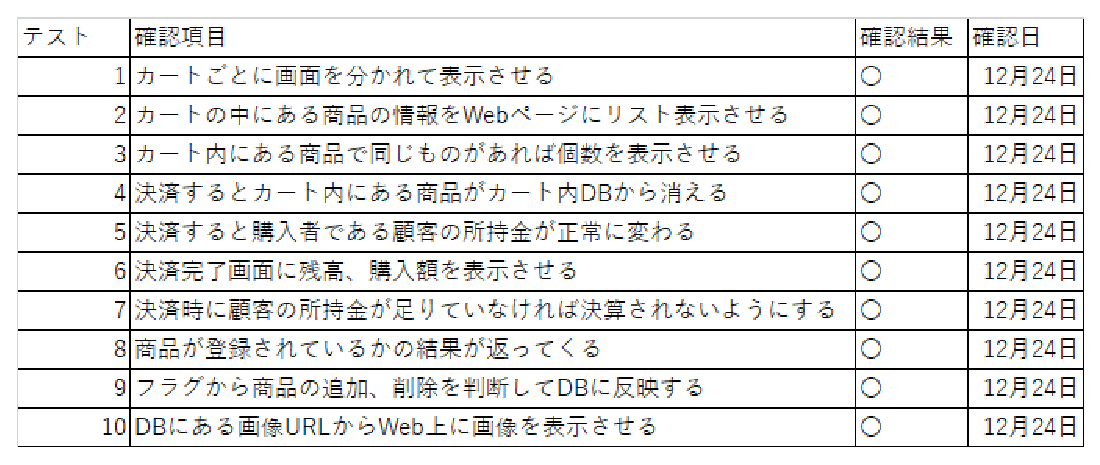
\includegraphics[width=15cm]{./pic/result/db_test_result.eps}
\label{db_test_result}
\end{table}

\newpage

\subsection{結合テスト}

これらの単体テストの項目を満たしていることを確認することで、商品識別システムが、表\ref{join_test_result}の結合テストの項目を満たしていることを確認する。結合テストでは、商品識別システムの中で筆者が実装を担当した、サーバ部分の項目が記されている。

\begin{table}[htbp]
\centering
\caption{結合テストの項目}
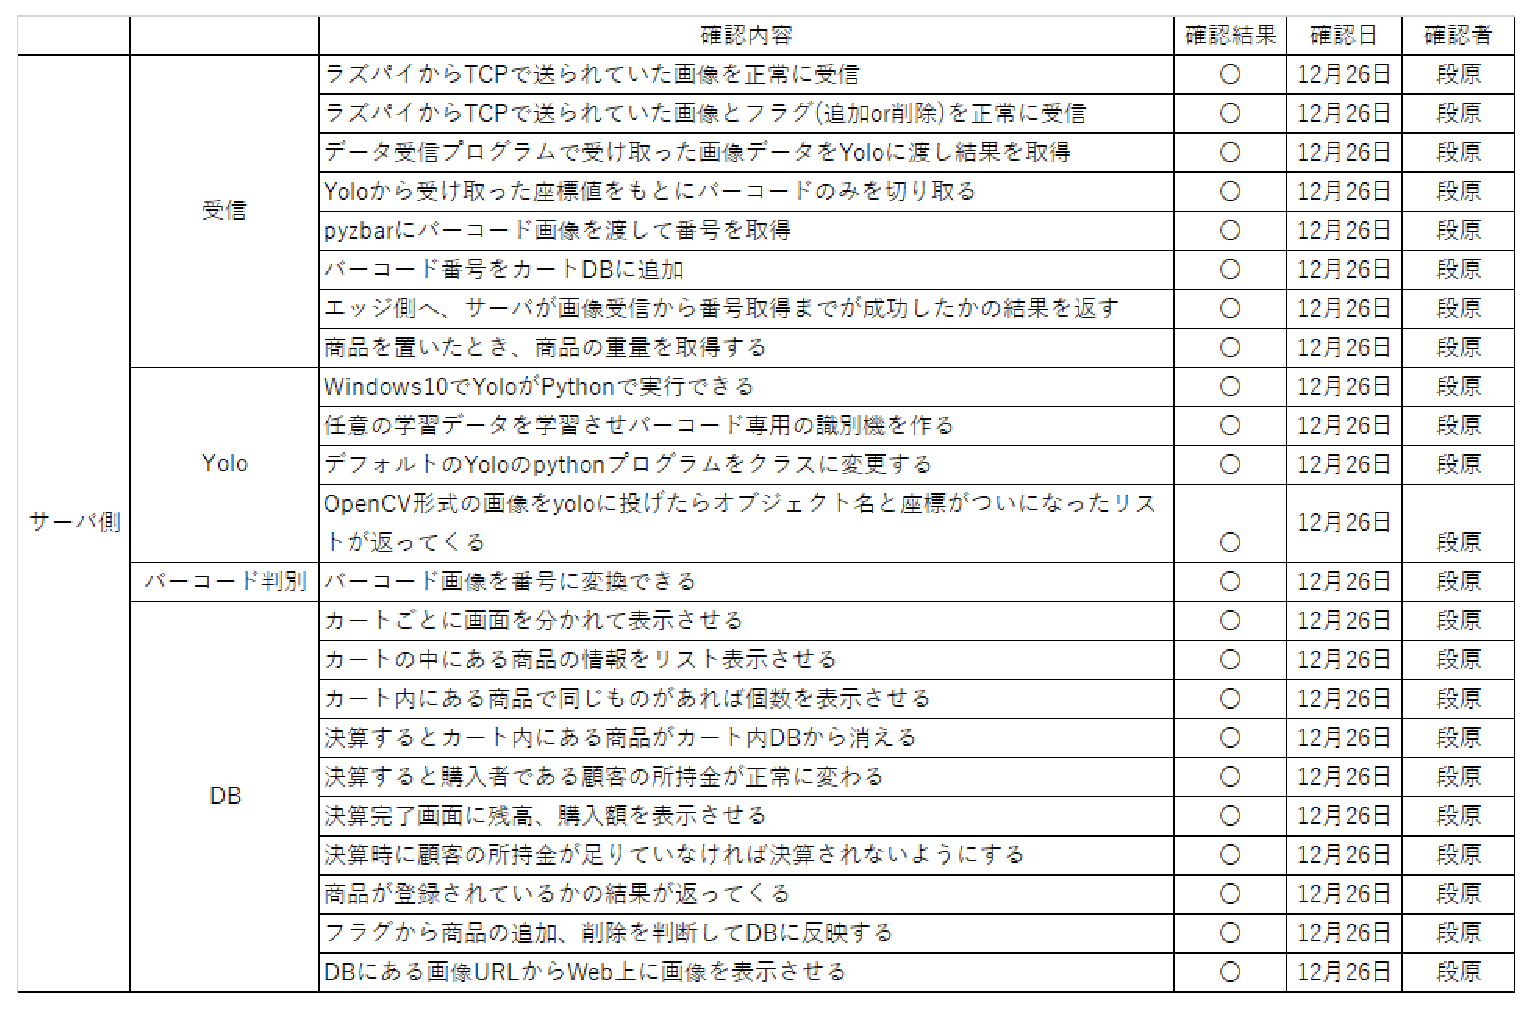
\includegraphics[height=15cm,width=15cm]{./pic/result/join_test_result.eps}
\label{join_test_result}
\end{table}

\newpage

\subsection{総合テスト}

結合テストの結果を確認し、各モジュール間でのデータの受け渡しが、正常に行われていることを確認した。最後に、表\ref{integrated_test_result}に総合テストの項目を示す。総合テストでは、ユーザが買い物を始めてから、決済するまでの流れをシナリオとしている。このシナリオでは、ユーザの残高は購入金額を下回らないと仮定する。また、決済前に買い物自体をキャンセルすることはないと仮定とした。

\begin{table}[htbp]
\centering
\caption{総合テストの項目}
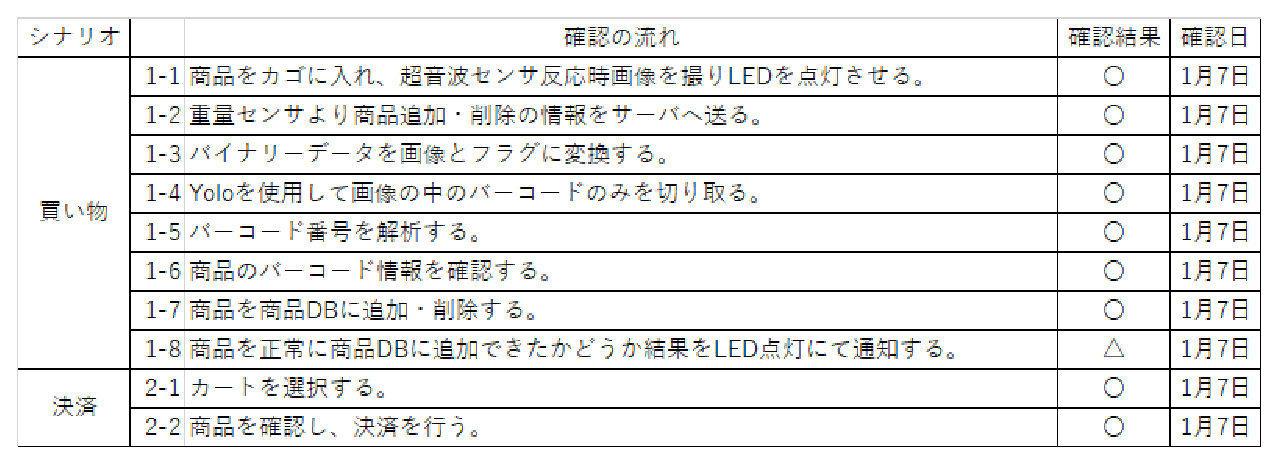
\includegraphics[width=15cm]{./pic/result/integrated_test_result.eps}
\label{integrated_test_result}
\end{table}